\clearpage
\section{ Problem 3.}
In $\mathbb{R}^2$, the weighted inner product is given by
$$ \langle x, y \rangle = ax_1y_1 + bx_2y_2 $$
where $a$ and $b$ are positive. Find a weighted inner product such that
the graph represents a unit circle as
\begin{figure}[H]
    \centering
    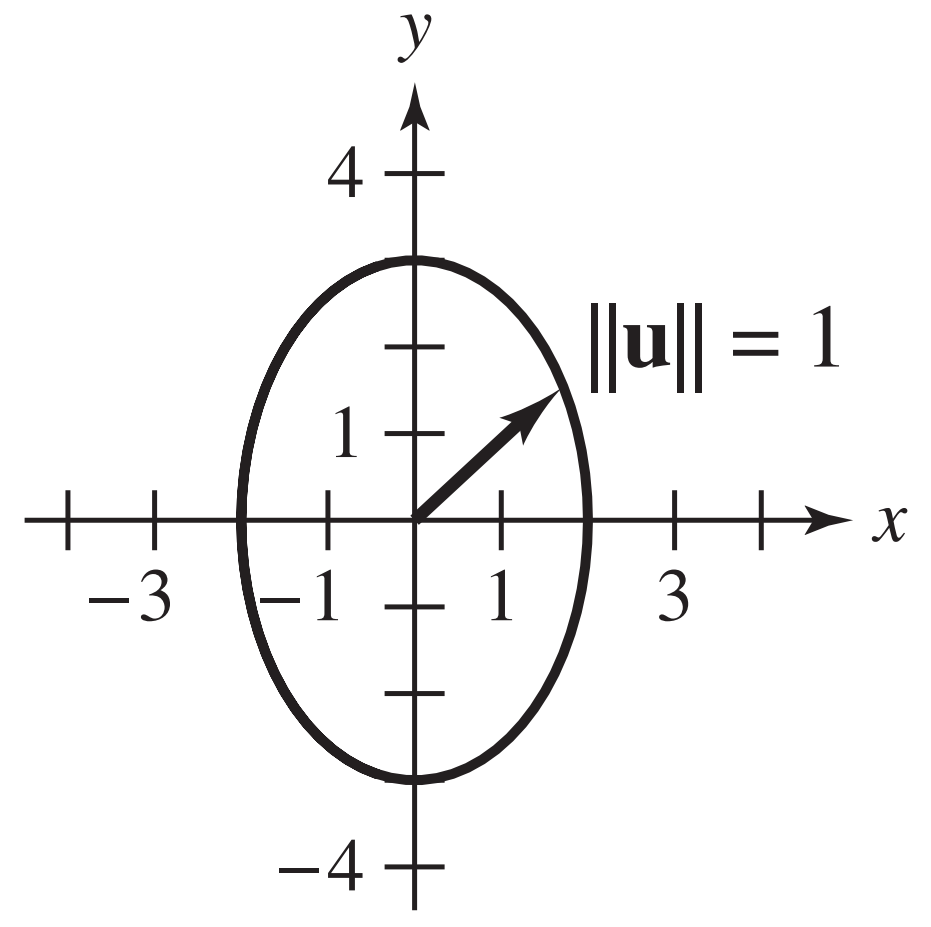
\includegraphics[width=6cm]{graphics/3_0.png}
    % \caption{}
\end{figure}
In that inner product space, reflect that unit circle about an input
plane.

\vspace*{1cm}

\textbf{Theory:}\\[6pt]
Weighted inner products have exactly the same algebraic properties
as the “ordinary” inner product. But they introduce weights or importance factors that modify the calculations and geometric interpretations. \\[6pt]
Let's consider a vector space $V$ over a field $F$. A weighted inner product on $V$ is a function that assigns a scalar value to each pair of vectors in $V$, incorporating weights or importance factors. Formally, a weighted inner product is defined as:
$$ \langle \cdot,\cdot \rangle_w : V \times V \rightarrow F $$
where $\langle \cdot,\cdot \rangle_w$ represents the weighted inner product, and $V \times V$ denotes the Cartesian product of $V$ with itself. \\[6pt]
In a weighted inner product, each component of the vector is multiplied by a corresponding weight or importance factor before the dot product is calculated. This allows for a more flexible and nuanced treatment of vector spaces, where certain components or dimensions may carry more significance or contribute differently to the overall computation. \\[6pt]

In order to solve this problem, we need to first find the weighted inner product such that the graph represents a unit circle. Then, we need to reflect that unit circle about an input plane.\\[6pt]

\vspace*{1cm}

\textbf{Python code:}
\lstinputlisting[language=Python]{code/problem3.py}

\clearpage

\textbf{Result:}
\begin{figure}[H]
    \centering
    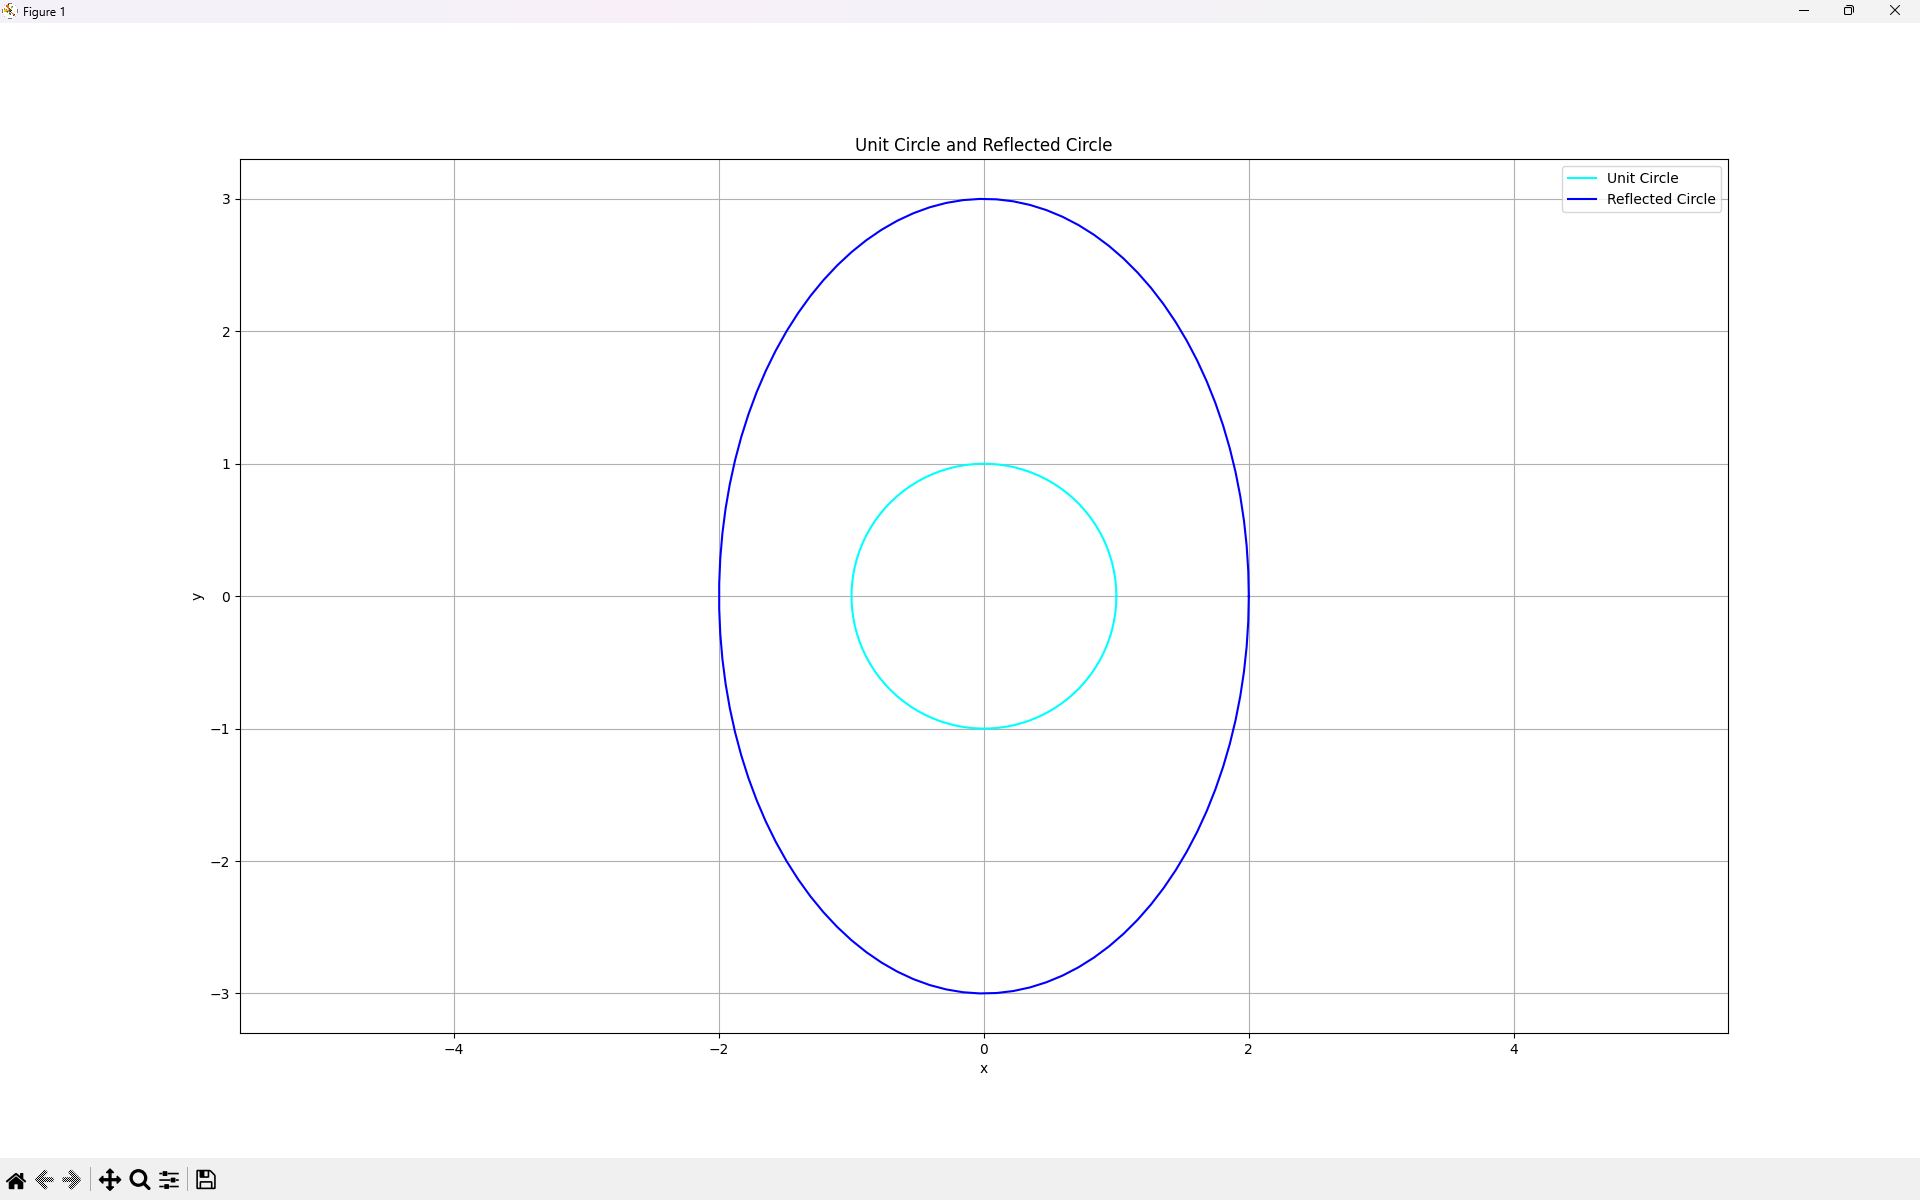
\includegraphics[width=16cm]{graphics/3.png}
    \caption*{Unit Circle and its reflection about the input plane}
\end{figure}